\documentclass[tikz, crop, border = {2pt 2pt 2pt 2pt}]{standalone}

\usepackage{physics}
\usetikzlibrary{decorations.pathreplacing, calligraphy}

\usepackage{unicode-math}
\setmathfont{Concrete-Math.otf}

\begin{document}
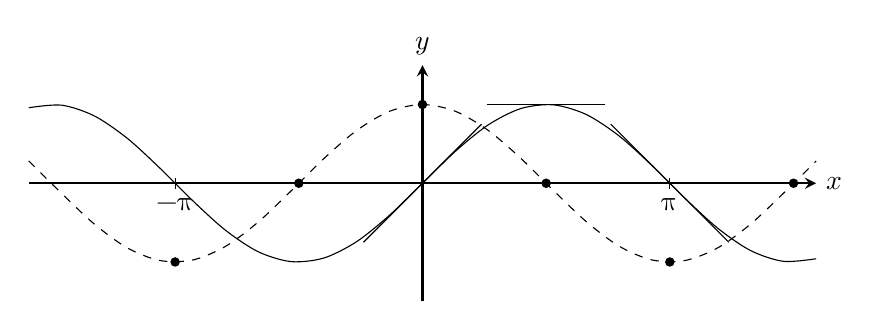
\begin{tikzpicture}
    \draw[-stealth, thick] (-5, 0) -- (5, 0) node[right]{$x$};
    \draw[-stealth, thick] (0, -1.5) -- (0, 1.5) node[above]{$y$};

    \draw[domain = -5:5, smooth] plot (\x, {sin(\x r)});
    \draw[domain = -5:5, smooth, dashed] plot (\x, {cos(\x r)});
    \draw ({pi}, 2pt) -- ++ (0, -4pt) node[below]{$\symrm{\pi}$};
    \draw ({-pi}, 2pt) -- ++ (0, -4pt) node[below]{$-\symrm{\pi}$};

    \draw (-0.75, -0.75) -- (0.75, 0.75);
    \draw ({pi/2 - 0.75}, 1) -- ++ (1.5, 0);
    \draw ({pi -0.75}, 0.75) -- ++ (1.5, -1.5);

    \filldraw (0, 1) circle (1.5pt);
    \filldraw ({pi/2}, 0) circle (1.5pt);
    \filldraw ({pi}, -1) circle (1.5pt);
    \filldraw ({3*pi/2}, 0) circle (1.5pt);
    \filldraw ({-pi/2}, 0) circle (1.5pt);
    \filldraw ({-pi}, -1) circle (1.5pt);
\end{tikzpicture}
\end{document}